\documentclass[tikz,border=10pt]{standalone}
\usepackage{tikz}
\usetikzlibrary{shapes.geometric, arrows.meta, positioning}

\tikzset{
    register/.style={
        rectangle, draw=black, thick,
        minimum width=1.2cm, minimum height=0.8cm,
        fill=white, font=\small\ttfamily
    },
    wire/.style={draw=black, thick, -Stealth},
    bus/.style={draw=black, line width=1.5pt, -Stealth},
    controlwire/.style={draw=black!60, dashed, -Stealth},
    buswidth/.style={font=\tiny, fill=white, inner sep=1pt},
    logic/.style={
        rectangle, draw=black, thick, rounded corners=3pt,
        minimum width=0.9cm, minimum height=0.8cm,
        fill=gray!10, font=\small
    }
}

\begin{document}
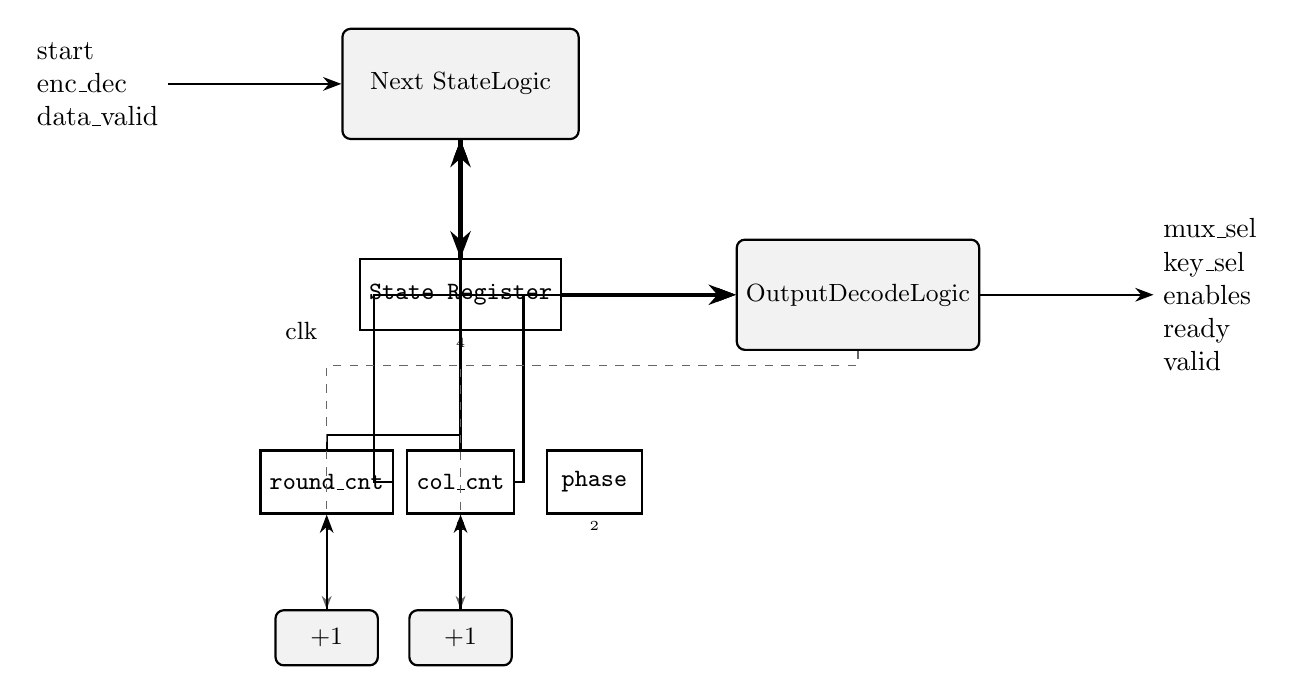
\begin{tikzpicture}[node distance=1.2cm and 1.8cm]

% State register (center)
\node[register, minimum width=2.3cm, minimum height=0.9cm] (state) at (0,0) {State Register};
\node[buswidth, below=0.05cm of state.south] {4};
\node[font=\small, left=0.4cm of state.south west] {clk};

% Next state logic (above)
\node[logic, above=1.5cm of state, minimum width=3cm, minimum height=1.4cm] (nsl) {Next State\\Logic};

% Output/decode logic (right)
\node[logic, right=2.2cm of state, minimum width=3cm, minimum height=1.4cm] (out) {Output\\Decode\\Logic};

% Counters (below state)
\node[register, below=1.5cm of state, xshift=-1.7cm, minimum width=1.3cm, minimum height=0.8cm] (rc) {round\_cnt};
\node[buswidth, below=0.05cm of rc.south] {4};

\node[register, below=1.5cm of state, xshift=0cm, minimum width=1.3cm, minimum height=0.8cm] (cc) {col\_cnt};
\node[buswidth, below=0.05cm of cc.south] {2};

\node[register, below=1.5cm of state, xshift=1.7cm, minimum width=1.2cm, minimum height=0.8cm] (ph) {phase};
\node[buswidth, below=0.05cm of ph.south] {2};

% Increment logic
\node[logic, below=1.2cm of rc, minimum width=1.3cm, minimum height=0.7cm] (inc1) {+1};
\node[logic, below=1.2cm of cc, minimum width=1.3cm, minimum height=0.7cm] (inc2) {+1};

% External inputs (left)
\node[left=2.2cm of nsl, font=\normalsize, align=left] (inputs) {start\\enc\_dec\\data\_valid};

% Control outputs (right)
\node[right=2.2cm of out, font=\normalsize, align=left] (outputs) {mux\_sel\\key\_sel\\enables\\ready\\valid};

% Dataflow connections
\draw[bus] (state) -- (nsl);
\draw[bus] (nsl) -- (state);
\draw[bus] (state) -- (out);

\draw[wire] (rc) -- ++(0,0.6) -| (nsl);
\draw[wire] (cc) -- ++(0,0.8) -| (nsl);
\draw[wire] (rc) -- ++(0.6,0) |- (out);
\draw[wire] (cc) -- ++(0.8,0) |- (out);

% Counter control
\draw[controlwire] (out) -- ++(0,-0.9) -| (inc1.north);
\draw[controlwire] (out) -- ++(0,-0.9) -| (inc2.north);
\draw[wire] (inc1) -- (rc);
\draw[wire] (inc2) -- (cc);

% External connections
\draw[wire] (inputs) -- (nsl);
\draw[wire] (out) -- (outputs);

\end{tikzpicture}
\end{document}
